\section{Event Reconstruction}
\label{sec:recon}

The event reconstruction software has been designed and developed within the CLARA framework. As discussed
in Section~\ref{sec:framework}, the reconstruction of events for CLAS12 is separated into micro-services that
execute data processing algorithms.

%%%%%%%%%%%%%%%%%%%%%%%%%%%%%%%%%%%%%%%%%%%%%%%%%%%%%%%%%%
\begin{figure*}
\centering
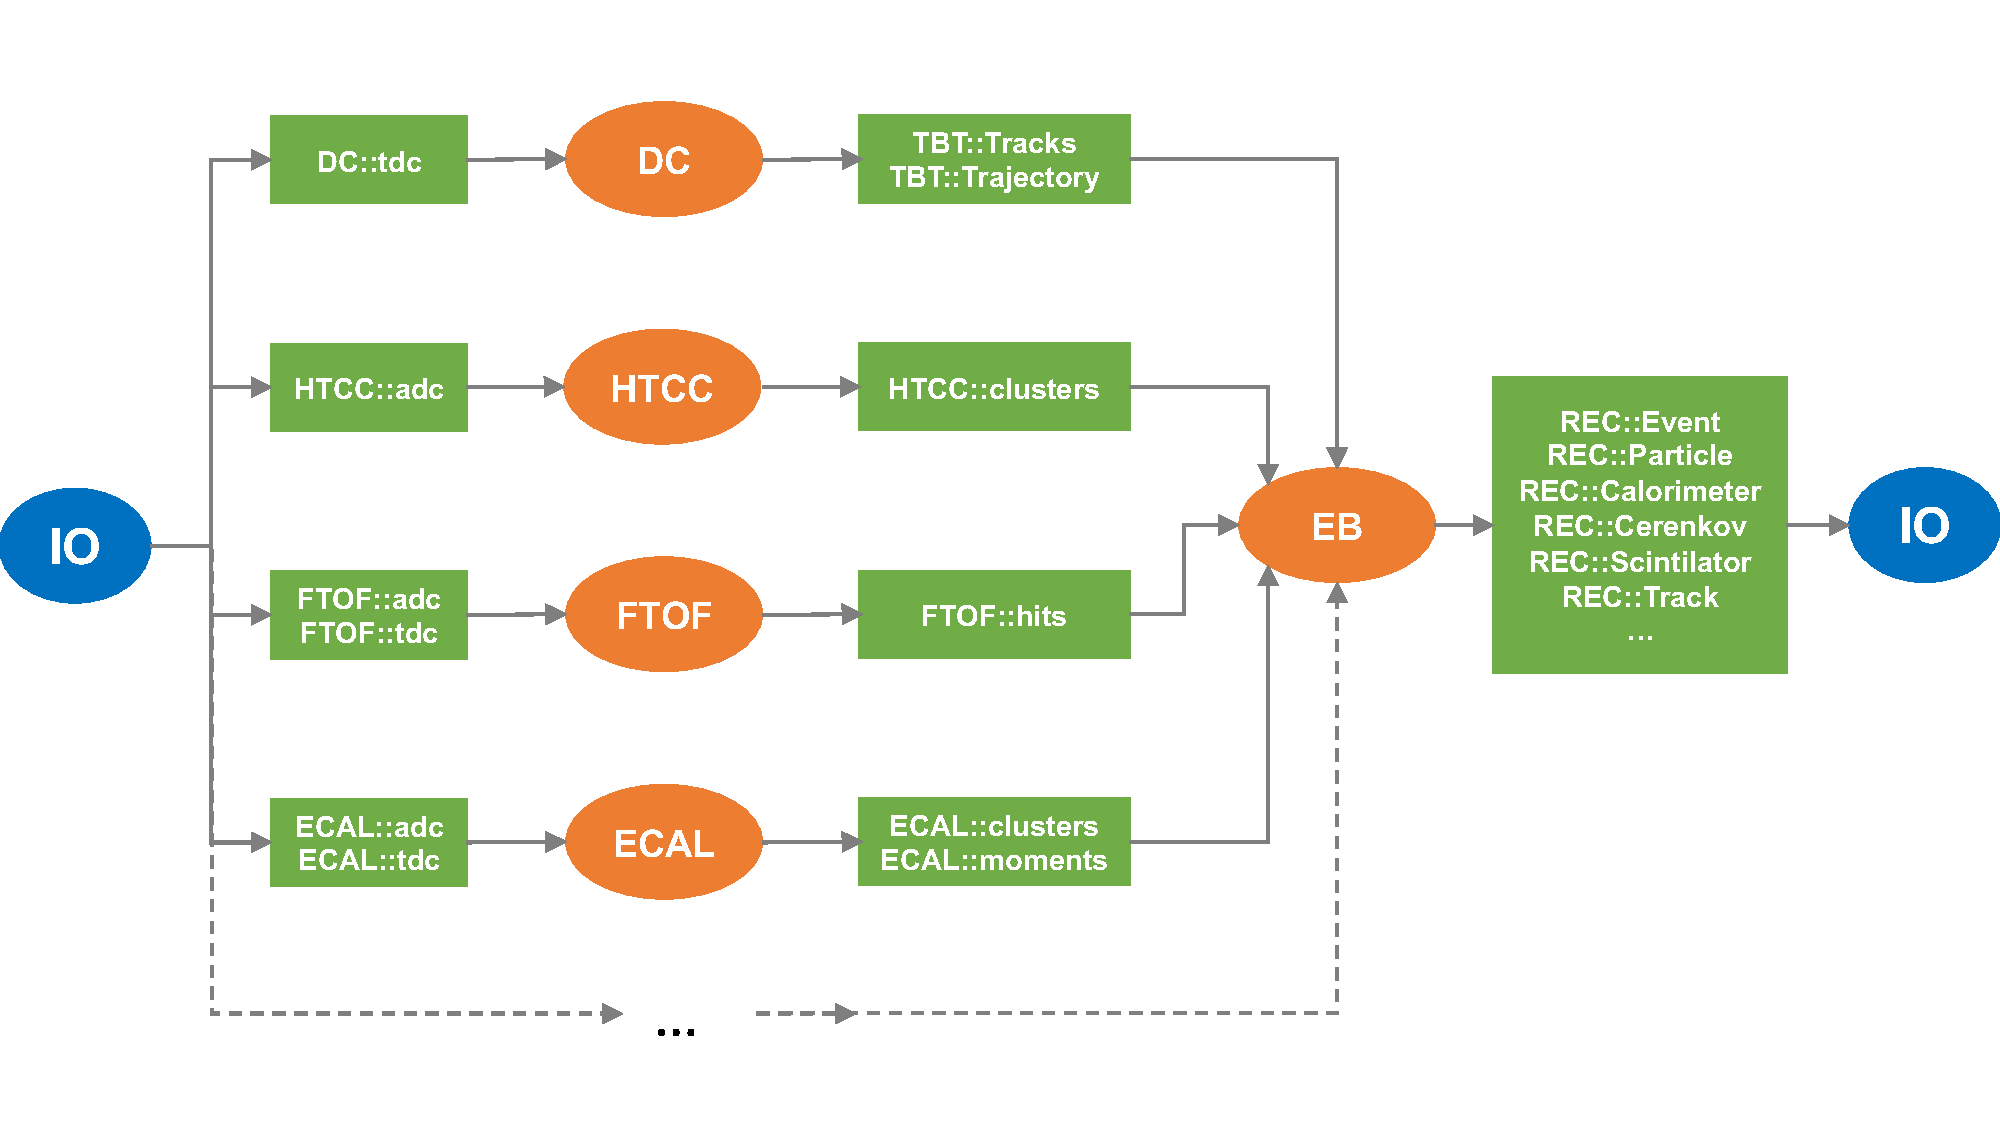
\includegraphics[width=0.85\textwidth]{pics/ServiceComposition.pdf}
\caption{Graphical representation of the CLAS12 interdependencies between services and banks. The I/O service
  reads events from the input file and distributes them to the reconstruction services chain for processing. Each
  service reads the relevant banks, applies the reconstruction algorithm, and provides output banks that are passed
  to the next service in the chain. The Event Builder (EB) service is executed as last in the chain; it collects the
  relevant banks from all CLAS12 subsystems services and produces event, particle, and detector response banks
  that are written to the output file.}
\label{fig:services}
\end{figure*}
%%%%%%%%%%%%%%%%%%%%%%%%%%%%%%%%%%%%%%%%%%%%%%%%%%%%%%%%%%%

The data reader services access the detector decoded data stored in banks (see Section~\ref{sec:framework}).
Each entry for the decoded detector hits is a row in a bank. A row includes detector element identifiers (sector,
layer, component, and order), and digitized detector data, such as signal charge, amplitude, time, or pedestal,
depending on the specific system. Similar bank structures are created at the decoding stage for the various
quantities needed for event reconstruction, such as hits, clusters, tracks, etc. The micro-services that implement
the reconstruction algorithms pertaining to the CLAS12 subsystems fill these banks, which are subsequently
appended and written out to a file by a data-persistency micro-service.

The services running the reconstruction algorithms access the various banks (transient data) as input and produce
output banks needed for the subsequent algorithms in the reconstruction chain. The order in which the services are
chained reflects the overall CLAS12 event reconstruction sequence and subsystem dependencies. First, charged
particle tracks are reconstructed in both the Central and Forward Detector tracking systems based on the position
of the recorded hits in the different detectors (i.e. using strip positions or wire locations). This procedure is
referred to as ``hit-based'' tracking. In parallel, hits recorded in the other detectors are processed to reconstruct
the energy and time of the associated particle interaction. These are matched to the reconstructed tracks by the
Event Builder service, based {\color{red} on hit position and time information}; unmatched hits are retained as neutral particle
candidates. At this stage, the Event Builder can reconstruct the event ``start time'', i.e. the time of the interaction
between the beam and target, and identify the reconstructed particles. Once the event start time is determined, a
second iteration of forward tracking can be performed to implement the so-called ``time-based'' tracking (which
also incorporates the drift times in the Drift Chambers). See Section~\ref{sec:hitrecon} for more details on
hit-based and time-based tracking.

The improved particle tracks from time-based tracking are the input for a second pass of the Event Builder, which
leads to the final event reconstruction. Given this sequence, some services can run in parallel, while others need the
reconstruction output provided by the preceding steps. For instance, hit-based tracking for the Central Vertex
Tracker (CVT) using the CVT service and for the Drift Chambers using the DCHB service (``HB'' is for hit-based)
can run in parallel, while time-based tracking for the Drift Chambers using the DCTB service {\color{red} (``TB'' is for time-based)}
must come after the first execution of the Event Builder service. An overview of the reconstruction application service
composition detailing these dependencies is shown in Fig.~\ref{fig:services}.
